%%%%%%%%%%%%%%%%%%%%%%%%%%%%%%%%%%%%%%%%%
% Short Sectioned Assignment LaTeX Template Version 1.0 (5/5/12)
% This template has been downloaded from: http://www.LaTeXTemplates.com
% Original author:  Frits Wenneker (http://www.howtotex.com)
% License: CC BY-NC-SA 3.0 (http://creativecommons.org/licenses/by-nc-sa/3.0/)
%%%%%%%%%%%%%%%%%%%%%%%%%%%%%%%%%%%%%%%%%

%----------------------------------------------------------------------------------------
%	PACKAGES AND OTHER DOCUMENT CONFIGURATIONS
%----------------------------------------------------------------------------------------

\documentclass[paper=a4, fontsize=11pt]{scrartcl} % A4 paper and 11pt font size

% ---- Entrada y salida de texto -----

\usepackage[T1]{fontenc} % Use 8-bit encoding that has 256 glyphs
\usepackage[utf8]{inputenc}
%\usepackage{fourier} % Use the Adobe Utopia font for the document - comment this line to return to the LaTeX default


\usepackage[utf8]{inputenc}
\usepackage[T1]{fontenc}
\usepackage[spanish]{babel}
\usepackage{times}

\usepackage{color}
\definecolor{gray97}{gray}{.97}
\definecolor{gray75}{gray}{.75}
\definecolor{gray45}{gray}{.45}

\usepackage{listings}
\lstset{ frame=Ltb,
	framerule=0pt,
	aboveskip=0.5cm,
	framextopmargin=3pt,
	framexbottommargin=3pt,
	framexleftmargin=0.4cm,
	framesep=0pt,
	rulesep=.4pt,
	backgroundcolor=\color{gray97},
	rulesepcolor=\color{black},
	%
	stringstyle=\ttfamily,
	showstringspaces = false,
	basicstyle=\small\ttfamily,
	commentstyle=\color{gray45},
	keywordstyle=\bfseries,
	%
	numbers=left,
	numbersep=15pt,
	numberstyle=\tiny,
	numberfirstline = false,
	breaklines=true,
}

% minimizar fragmentado de listados
\lstnewenvironment{listing}[1][]
{\lstset{#1}\pagebreak[0]}{\pagebreak[0]}

\lstdefinestyle{consola}
{basicstyle=\scriptsize\bf\ttfamily,
	backgroundcolor=\color{gray75},
}

\lstdefinestyle{C}
{language=C,
}
% ---- Idioma --------

\usepackage[spanish, es-tabla]{babel} % Selecciona el español para palabras introducidas automáticamente, p.ej. "septiembre" en la fecha y especifica que se use la palabra Tabla en vez de Cuadro
% ---- Otros paquetes ----

\usepackage{amsmath,amsfonts,amsthm} % Math packages
%\usepackage{graphics,graphicx, floatrow} %para incluir imágenes y notas en las imágenes
\usepackage{graphics,graphicx, float} %para incluir imágenes y colocarlas

% Para hacer tablas comlejas
%\usepackage{multirow}
%\usepackage{threeparttable}

%\usepackage{sectsty} % Allows customizing section commands
%\allsectionsfont{\centering \normalfont\scshape} % Make all sections centered, the default font and small caps

\usepackage{fancyhdr} % Custom headers and footers
\pagestyle{fancyplain} % Makes all pages in the document conform to the custom headers and footers
\fancyhead{} % No page header - if you want one, create it in the same way as the footers below
\fancyfoot[L]{} % Empty left footer
\fancyfoot[C]{} % Empty center footer
\fancyfoot[R]{\thepage} % Page numbering for right footer
\renewcommand{\headrulewidth}{0pt} % Remove header underlines
\renewcommand{\footrulewidth}{0pt} % Remove footer underlines
\setlength{\headheight}{13.6pt} % Customize the height of the header

\numberwithin{equation}{section} % Number equations within sections (i.e. 1.1, 1.2, 2.1, 2.2 instead of 1, 2, 3, 4)
\numberwithin{figure}{section} % Number figures within sections (i.e. 1.1, 1.2, 2.1, 2.2 instead of 1, 2, 3, 4)
\numberwithin{table}{section} % Number tables within sections (i.e. 1.1, 1.2, 2.1, 2.2 instead of 1, 2, 3, 4)

\setlength\parindent{0pt} % Removes all indentation from paragraphs - comment this line for an assignment with lots of text

\newcommand{\horrule}[1]{\rule{\linewidth}{#1}} % Create horizontal rule command with 1 argument of height


\begin{document}
\title{
\normalfont \normalsize 
\textsc{{\bf Aprendizaje Automático (2015-16) \\ Grado en Ingeniería Informática \\ Universidad de Granada} \\ [25pt] % Your university, school and/or department name(s)
\horrule{0.5pt} \\[0.4cm] % Thin top horizontal rule
\huge Informe Trabajo de Prácticas 2 \\ % The assignment title
\horrule{2pt} \\[0.5cm] % Thick bottom horizontal rule
}}
\author{Miguel López Campos} % Nombre y apellidos

\date{\normalsize\today} % Incluye la fecha actual
%----------------------------------------------------------------------------------------
% DOCUMENTO
%----------------------------------------------------------------------------------------


	
	\maketitle % Muestra el Título
	\newpage %inserta un salto de página
	\tableofcontents % para generar el índice de contenidos
	\listoffigures

	
	\newpage
	
	\
	
	\section{Modelos Lineales}
		\subsection{Ejercicio 1}
		 \textbf{Gradiente Descendente}. Implementar el algoritmo de gradiente descendente.
		\begin{enumerate}
			\item \label{1} Considerar la función no lineal de error $E(u,v)=(ue^v-2ve^{-u})^2$. Usar gradiente descendente y minimizar esta función de error, comenzando desde el punto $(u,v)=(1,1)$ y usando una tasa de aprendizaje $\eta=0.1$.
			\\
			\\
			
			Para implementar gradiente descendente he realizado varias versiones. En la más genérica lo que hago es poner como criterio de parada que la diferencia entre el punto anteriormente calculado y el actual sea menor que un umbral y que el número de iteraciones del algoritmo no supere un máximo dado como argumento. También tendrá como argumento la función (la cual devolverá tanto la evaluación de la función en el punto dado como un vector de argumentos, así como el gradiente) y la tasa de aprendizaje.
			\\
			\\
			
			El algoritmo lo que hace básicamente es actualizar los pesos con la regla $w_{t+1}=w_{t}-\eta \bigtriangledown E $
			\begin{enumerate}
				\item Calcular analíticamente y mostrar la expresión del gradiente de la función $E(u,v)$
				\\
				\\
				Cáculo analítico del gradiente:
				\\
				
				$$\frac{\delta E}{\delta u} = 2(ue^{v}-2ve^{-u})(e^{v}+2ve^{-u})$$
				\\
				$$\frac{\delta E}{\delta v} = 2(ue^{v}-2ve^{-u})(ue^{v}-2e^{-u})$$
				\item ¿Cuántas iteraciones tarda el algoritmo en obtener por primera vez un valor de $E(u,v)$ inferior  a $10^{-14}$ . (Usar flotantes de 64 bits)
				
				\item ¿Qué valores de $(u,v)$ obtuvo en el apartado anterior cuando alcanzó el error de $10^{-14}$.
				\begin{figure} [H]
				\centering
				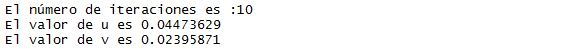
\includegraphics[width=0.7\linewidth]{captura1}
				\caption{Iteraciones antes de llegar al umbral y valor de las variables}
				\label{fig:captura1}
				\end{figure}
				
				Como vemos en la figura anterior, los resultados de las variables son muy cercanas a 0 (tanto u como v). Esto es porque el mínimo se encuentra en (0,0). El algoritmo no alcanza la solución exacta pero aún así nos da una aproximación buena. 

			\end{enumerate}
			%
			\item \label{gd} Considerar ahora la función $f(x,y)=x^2+2y^2+2\sin(2\pi x)\sin(2\pi y)$
			\begin{enumerate}
				\item Usar gradiente descendente para minimizar esta función. Usar como valores iniciales $x_0=1,y_0=1$, la tasa de aprendizaje $\eta=0.01$ y un máximo de 50 iteraciones. Generar un gráfico de cómo desciende el valor de la función con las iteraciones. Repetir el experimento pero usando $\eta=0.1$, comentar las diferencias.
				\begin{figure} [H]
				\centering
				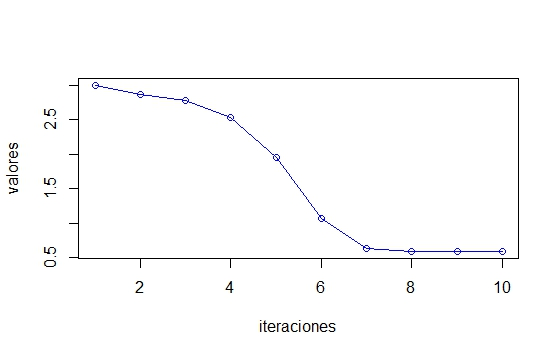
\includegraphics[width=0.7\linewidth]{captura2}
				\caption{Gráfica para tasa=0.01}
				\label{fig:captura2}
				\end{figure}
				
				\begin{figure} [H]
				\centering
				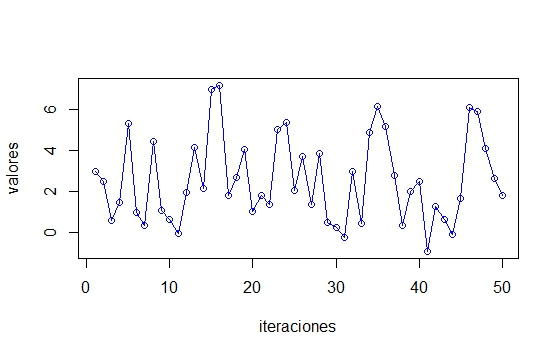
\includegraphics[width=0.7\linewidth]{captura3}
				\caption{Gráfica para tasa=0.1}
				\label{fig:captura3}
				\end{figure}

			Como vemos las diferencias son significativas. Mientras que con la tasa puesta a 0.01 converge toda la gráfica a un mismo valor, con 0.1 en cambio la gráfica fluctúa mucho. Esto es debido a que la función a la que hemos aplicado gradiente descendente tiene senos y cosenos, por lo que tiene muchos máximos y mínimos (fluctúa mucho). Cuando aumentamos la tasa de aprendizaje lo que hacemos es "aumentar el vector gradiente", lo que hace que si estamos en un mínimo local o global, sea más posible salir de él debido a que el vector gradiente es más grande.

				\item Obtener el valor mínimo y los valores de las variables que lo alcanzan cuando el punto de inicio se fija: $(0.1,0.1)$, $(1,1)$,$(-0.5,-0.5)$,$(-1,-1)$. Generar una tabla con los valores obtenidos ¿Cuál sería su conclusión sobre la verdadera dificultad de encontrar el mínimo global de una función arbitraria?
				
				\begin{figure} [H]
				\centering
				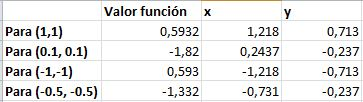
\includegraphics[width=0.7\linewidth]{Captura4}
				\caption{Tabla resultados de gradiente descendente}
				\label{fig:Captura4}
				\end{figure}
				
				Para la ejecución he usado un número máximo de iteraciones igual a 50 y una tasa de aprendizaje de 0.01. Como vemos los resultados son muy diversos. Esto se debe a que la función a la cual le hemos calculado el mínimo, es muy variable (tiene funciones trigonométricas). Por lo tanto, el punto inicial en el que empecemos a aplicar gradiente descendente puede ser muy importante a la hora de los resultados.

			\end{enumerate}
			
			\subsection{Ejercicio 2}
			 \textbf{Coordenada descendente}. En este ejercicio comparamos la eficiencia de la técnica de optimización de ``coordenada descendente'' usando la misma función del ejercicio 1. En cada iteración, tenemos dos pasos a lo largo de dos coordenadas. En el Paso-1 nos movemos a lo largo de la coordenada $u$ para reducir el error (suponer que se verifica una aproximación de primer orden como en gradiente descendente), y  el Paso-2 es para reevaluar y movernos a lo largo de la coordenada $v$ para reducir el error ( hacer la misma hipótesis que en el paso-1). Usar una tasa de aprendizaje $\eta=0.1$.
			 
			 La implementación la he hecho con el siguiente código.
			 \begin{lstlisting}
coordenada_descendente <- function(funcion, inicio, tasa=0.1, max_iters)
{
	ant <- 500.0
	w <- inicio
	act <- 0.0
	iters <- 0
	
	##Criterio de parada. Mientras el valor de la función en la anterior iteración 
	##y el de la actual sean prácticamente iguales (según el umbral)
	while(iters < max_iters)
	{
		ant <- act
		resultados <- funcion(w)
		derivadas <- resultados[2:length(resultados)] 
		
		#Primero la coordenada u
		w[1] <- w[1] - tasa*derivadas[1]
		
		#Después la coordenada v
		resultados <- funcion(w)
		derivadas <- resultados[2:length(resultados)]
		w[2] <- w[2] - tasa*derivadas[2]
		
		##Obtengo el valor de la siguiente iteración
		resultados <- funcion(w)
		act <- resultados[1]
		
		iters <- iters+1
		
		}
	return (list(act,w,iters))
}
			 
			 \end{lstlisting}
			 \begin{enumerate}
			 	\item ¿Qué valor de la función $E(u,v)$ se obtiene después de 15 iteraciones completas (i.e. 30 pasos) ?
			 	\\
			 	u = 6.297
			 	\\
			 	v = -2.85
			 	\item Establezca una comparación entre esta técnica y la técnica de gradiente descendente.
			 	\\
			 	Según nuestro experimento, coordenada descendente nos da resultados mucho peores que gradiente descendente. Mientras que gradiente descendente con sólo 10 iteraciones ya nos daba una solución muy cercana a la real, en coordenada descendente en 15 iteraciones nos da una bastante peor. Quizás si se ejecutara más tiempo si llegaríamos a una buena solución.
			 \end{enumerate}
		\end{enumerate}
		
		
	\subsection{Ejercicio 3}
	 \textbf{Método de Newton} Implementar el algoritmo de minimización de Newton y aplicarlo a la función $f(x,y)$ dada en el ejercicio 1. Desarrolle los mismos experimentos usando los mismos puntos de inicio.
	 \\
	 En este ejercicio he tenido problemas (no sé por qué). En el dibujo de la gráfica aparece una gráfica un tanto extraña, en la que a partir de la segunda iteración la gráfica ya se mantiene constante en un mismo valor. La actualización de los pesos la he realizado con la fórmula $w_{t+1} = w_t -H^{-1}\nabla E_{in}(w_t})$ La implementación es la siguiente:
	 
	 \begin{lstlisting}
minimizacion_newton <- function(wini, umbral=10^-3, max_iters)
{
	ant <- 500.0
	w <- wini
	act <- 0.0
	iters <- 0
	
	
	valores <- vector()
	
	
	while(iters<max_iters)
	{
		ant <- act
		resultados <- funcionB(as.vector(w))
		# gradiente <- funcionB(wini)[2:length(resultados)]
		gradiente <- resultados[2:length(resultados)]
		
		
		valores[iters+1] <- resultados[1]
		#Creo la función H con las segundas derivadas
		value1 <- 2-8*pi^2*sin(2*pi*w[2])*sin(2*pi*w[1])
		value2 <- 8*pi^2*cos(2*pi*w[1])*cos(2*pi*w[2])
		value3 <- 8*pi^2*cos(2*pi*w[1])*cos(2*pi*w[2])
		value4 <- 4-8*pi^2*sin(2*pi*w[1])*sin(2*pi*w[2])
		
		fila1 <- c(value1, value2)
		fila2 <- c(value3, value4)
		
		H <- rbind(fila1, fila2)
		H_inversa <- solve(H)
		
		w <- w-H_inversa %*% gradiente
		
		iters <- iters+1
	}
	
	iteraciones <- 1:iters
	plot(x=iteraciones, y=valores, type="o", col="blue")
	
	return(list(ant,w,iters))
}
	 \end{lstlisting}
	 
	 La implementación en teoría está bien. La matriz hessiana está bien calculada (lo he comprobado con la función hessian) así como su inversa. El gráfico lo podemos ver en la siguiente figura.
	 \begin{itemize}
	 	\item Generar un gráfico de como desciende el valor de la función con las iteraciones.
	 	
	 	Para ejecutarlo he puesto un máximo de iteraciones de 10. Al principio puse más pero al ver que se mantenía constante al final, dejé 10.
	 	
	 	\begin{figure} [H]
		\centering
		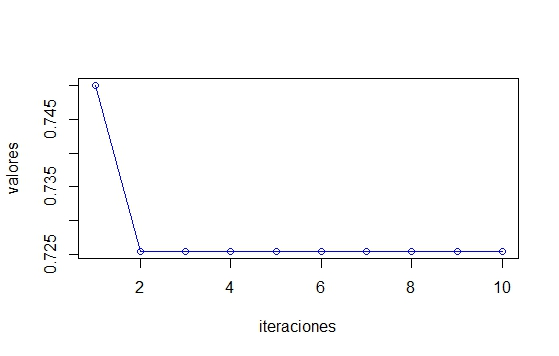
\includegraphics[width=0.7\linewidth]{captura5}
		\caption{Variación del valor de la función con las iteraciones. Para (-0.5,-0.5)}
		\label{fig:captura5}
		\end{figure}
		
		\begin{figure} [H]
		\centering
		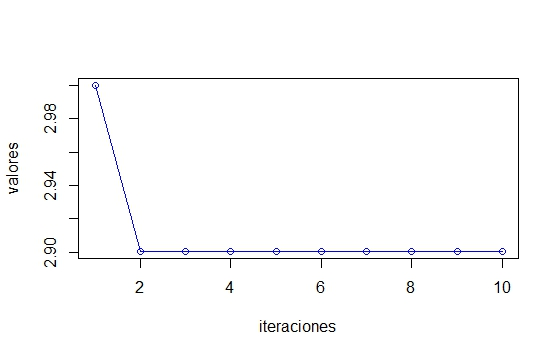
\includegraphics[width=0.7\linewidth]{captura6}
		\caption{Para (-1,-1)}
		\label{fig:captura6}
		\end{figure}
		
		\begin{figure} [H]
		\centering
		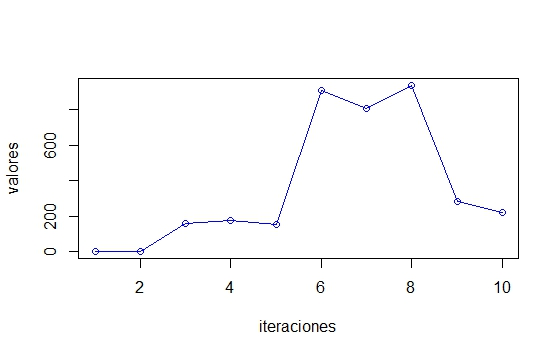
\includegraphics[width=0.7\linewidth]{captura7}
		\caption{Para (0.1,0.1)}
		\label{fig:captura7}
		\end{figure}
		
		\begin{figure} [H]
		\centering
		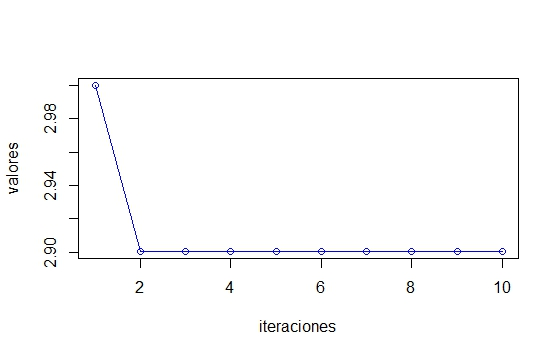
\includegraphics[width=0.7\linewidth]{captura8}
		\caption{Para (1,1)}
		\label{fig:captura8}
		\end{figure}




	 	\item Extraer conclusiones sobre las conductas de los algoritmos comparando  la curva de decrecimiento de la función calculada en el apartado anterior y la correspondiente obtenida con gradiente descendente.
	 	\\
	 	\\
	 	De mis gráficas (aunque creo que no están bien) puedo decir que el método de Newton da un resultado bastante peor. En todas menos para los valores iniciales 0.1,0.1 presenta un comportamiento que a partir de la segunda iteración se mantiene constante (y siempre con valores de la función más altos que en gradiente descendente). En 0.1,0.1 hay más movimiento en el comportamiento pero el resultado es mucho peor que el que gradiente descendente nos da.
	 \end{itemize}
	 
	 
	 \subsection{Ejercicio 4}
	 \textbf{Regresión Logística}: En este ejercicio crearemos  nuestra propia función objetivo $f$ (probabilidad en este caso) y nuestro conjunto de datos $\calD$ para ver cómo funciona regresión logística. Supondremos por simplicidad que $f$ es una probabilidad con valores $0/1$ y por tanto que $y$ es una función determinista de $\bfx$.
	 
	 Consideremos $d=2$ para que los datos sean visualizables, y sea $\mathrm{X=[-1,1]\times[-1,1]}$ con probabilidad uniforme de elegir cada $\mathrm{x \in X}$.  Elegir una línea en el plano como la frontera entre $f(x)=1$ (donde $y$ toma valores $+1$) y $f(x)=0$ (donde $y$ toma valores $-1$), para ello seleccionar dos puntos aleatorios del plano y calcular la línea que pasa por ambos. Seleccionar $N=100$ puntos aleatorios $\{x_n\}$ de $\calX$ y evaluar las respuestas de todos ellos $\{y_n\}$ respecto de la frontera elegida.
	 \begin{enumerate}
	 	\item Implementar Regresión Logística(RL) con Gradiente Descendente Estocástico (SGD) bajo las siguientes condiciones:
	 	\begin{itemize}
	 		\item Inicializar el vector de pesos con valores 0.
	 		\item Parar el algoritmo cuando $\mathrm{||w^{(t-1)}-w^{(t)}||<0.01}$, donde $w^{(t)}$ denota el vector de pesos al final de la época $t$. Una época es un pase completo a través de los $N$ datos. 
	 		\item Aplicar una permutación aleatoria de $1,2,\dots,N$ a los datos antes de usarlos en cada época  del algoritmo.
	 		\item Usar una tasa de aprendizaje de $\eta=0.01$
	 	\end{itemize}
	 	\\
	 	\\
	 	
	 	Primero genero una muestra aleatoria con distribución uniforme con N=100. Después lo que hago es etiquetar este conjunto de datos con una línea generada de forma aleatoria en el el cuadrado [-1,1]x[-1,1].
	 	\\
	 	
	 	La implementación de la regresión logística la he hecho con el siguiente código (gradiente estocástico):
	 	\newpage
	 	
	 	\begin{lstlisting}
gradiente_estocastico <- function(muestra, etiquetas, wini, umbral = 0.01, tasa = 0.01)
{

	w <- wini
	diferencia_modulo <- 10
	
	#Criterio de parada ||Want-W|| < umbral (0.01)
	while(diferencia_modulo >= umbral)
	{
		#Genero una "mezcla" de la muestra con la función sample.
		#Lo que hago es coger un vector de enteros que van desde el 1 hasta el número
		#de filas de muestra y sample los permuta aleatoriamente
		permutacion_aleatoria <- sample(x=(1:nrow(muestra)), size=nrow(muestra))
		want <- w
		
		#Para cada punto de la permutación aleatoria
		for(i in permutacion_aleatoria)
		{
			#Actualizo los pesos según el algoritmo de regresión logística
			w <- w - tasa*(-etiquetas[i]*muestra[i,])/(1+exp(etiquetas[i]*muestra[i,]*want))
		}
		
		#Calculo la diferencia de modulos
		#modulowant <- sqrt(sum(want))
		#modulow <- sqrt(sum(w))
		dif <- w-want
		diferencia_modulo <- sqrt(sum(dif^2))
	}

return(w)
}
	 	\end{lstlisting}
	 	\item Usar la muestra de datos etiquetada para encontrar $g$ y estimar $Eout$  usando para ello un número suficientemente grande de nuevas muestras. 
	 \end{enumerate}
	 	\\
	 	\\
	 	
	 	Para estimar g aplico regresión logística sobre el conjunto de datos generado. Los pesos iniciales que le doy son (0,0,0) y tanto el umbral (para el criterio de parada) como la tasa de aprendizaje la pongo a 0.01.
	 	\\
	 	\\
	 	
	 	Tras ejecutar el algoritmo y comprobar los pesos obtenidos, puedo ver que efectivamente se asemejan a los pesos de la función que hemos estimado. Para calcular el error uso el error de entropía cruzada:
	 	
	 	$$E_{out}=\frac{1}{N}\sum_{n=1}^{N}ln(1+e^{-y_{n}w^{T}x_{n}})$$
	 		
		Donde $x_n$ será el conjunto de datos nuevo e $y_n$ su etiquetado. En este experimento obtengo un $E_{out}=0.224$

	\subsection{Ejercicio 5}
	\textbf{Clasificación de Dígitos}. Considerar el conjunto de datos de los dígitos manuscritos y seleccionar las muestras de los dígitos 1 y 5. Usar los ficheros de entrenamiento (training) y test que se proporcionan. Extraer las características de {\bf intensidad promedio} y {\bf simetría} en la manera que se indicó en el ejercicio 3 del trabajo 1.
	
	Plantear un problema de clasificación binaria que considere el conjunto de entrenamiento como datos de entrada para aprender la función $g$. Usando el modelo de Regresión Lineal para clasificación seguido por PLA-Pocket como mejora. Responder a las siguientes cuestiones.
	\\
	\\
	Lo primero que tengo que hacer es leer los datos y adaptar las estructuras de datos para que tanto en el dataset de training como en el de test haya sólo 1's y 5's. Después saco la intensidad media y la simetría ayudándome de funciones.
	\\
	\\
	Para estimar la función he usado regresión lineal y posteriormente el pocket PLA (ya implementados en la primera práctica).
	
	\begin{enumerate}
		\item Generar gráficos separados (en color) de los datos de entrenamiento y test junto con la función estimada.
		\\
		\\
		A continuación la gráfica para el conjunto de training con la recta estimada.
		\begin{figure} [H]
		\centering
		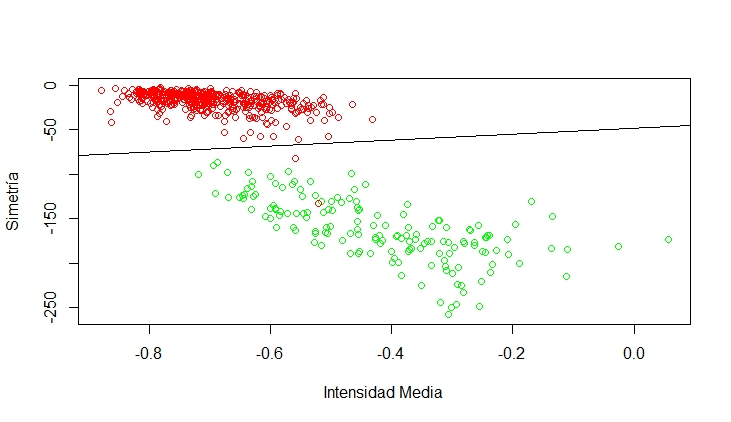
\includegraphics[width=1.0\linewidth]{captura9}
		\caption{Función estimada y datos de entrenamiento}
		\label{fig:captura9}
		\end{figure}
		
		Con el conjunto de test.
		\begin{figure} [H]
		\centering
		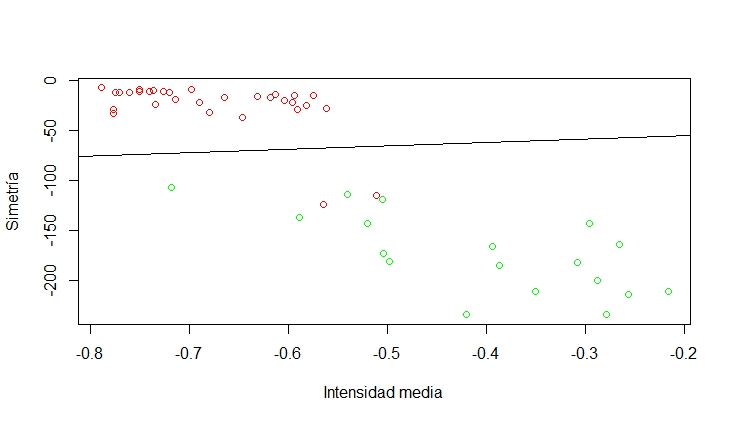
\includegraphics[width=1.0\linewidth]{captura10}
		\caption{Función estimada y datos de test}
		\label{fig:captura10}
		\end{figure}

		
		
		\item Calcular $E_{in}$ y $E_{test}$ (error sobre los datos de test).
		\\
		\\
		Para sacar $E_{in}$ y $E_{test}$, sólo tengo que dividir el número de fallos entre el total de muestra:
		El $E_{in}$ es del 0.3338898\%.
		\\
		El $E_{test}$ es del 4.082\%.
		\item Obtener cotas sobre el verdadero valor de $E_{out}$. Pueden calcularse dos cotas una basada en $E_{in}$ y otra basada en $E_{test}$. Usar una tolerancia $\delta=0.05$. ¿Que cota es mejor?
		\\
		\\
		
		Con el $E_{in}$ uso la fórmula:
		$$E_{out}(g) \leq E_{in}(g) + \sqrt{\frac{8}{N}ln(\frac{4((2N)^{d_{vc}}+1)}{\delta})}$$
		
		Sabemos que para 2D $d_{vc}=3$. Por lo tanto $E_{out} \leq 0.9183$.
	\end{enumerate}
	
	
	\section{Sobreajuste}
	\subsection{Ejercicio 1}
	\textbf{Sobreajuste.} Vamos a construir un entorno que nos permita experimentar con los problemas de sobreajuste. Consideremos el espacio de entrada $X=[-1,1]$ con una densidad de probabilidad uniforme, $P(x)=\frac{1}{2}$. Consideramos dos modelos $H_2$ y $H_{10}$ representando el conjunto de todos los polinomios de grado 2 y grado 10 respectivamente. La función objetivo es un polinomio de grado $Q_f$ que escribimos como $f(x)=\sum_{q=0}^{Q_f} a_q L_q(x)$, donde $L_q(x)$ son los polinomios de Legendre (ver la relación de ejercicios.2). El conjunto de datos es $D=\{ (x_1,y_1),s,(x_N,y_N)\}$ donde $y_n=f(x_n)+\sigma\epsilon_n$ y las $\{\epsilon_n\}$ son variables aleatorias i.i.d.  ${{N}}(0,1)$ y $\sigma^2$ la varianza del ruido.
	
	Comenzamos realizando un experimento donde suponemos que los valores  de $Q_f,N, \sigma$, están especificados, para ello:
	\begin{itemize}
		\item Generamos  los coeficientes $a_q$ a partir de muestras de una distribución ${{N}}(0,1)$ y escalamos dichos coeficientes de manera que $E_{\mathbf{a},x}[f^2]=1$ (Ayuda: Dividir los coeficientes por $\sqrt{\sum_{q=0}^{Q_f} \frac{1}{2q+1}}$ )
		\item Generamos un conjunto de datos,  $x_1,\dots,x_N$ muestreando de forma independiente  $P(x)$ y los valores $y_n=f(x_n)+\sigma\epsilon_n$.
	\end{itemize}
	\\
	\\
	
	Para la función f he implementado la siguiente función:
	\begin{lstlisting}
	
#Esta es la función f
funcionF <- function(x, Qf)
{
	suma <- 0.0
	#Sumatoria
	for(i in 0:Qf)
	{
		a <- 0:Qf
		aq <- rnorm(n=1, mean=0, sd=1)
		aq <- aq/(sqrt(sum(1/(2*a+1))))
		#slegendre.polynomials nos devuelve una lista de objetos polynomials
		#que corresponden con los polinomios de Legendre desde k=0 hasta k dado como
		#argumento. al hacer as.function se transforma la clase polynomial a una función
		#la cual evaluaremos sobre x
		L <- as.function(legendre.polynomials(i)[[i+1]])
		suma <- suma+aq*L(x)
	}
	
	return(suma)
}
	\end{lstlisting}
	La función legendre.polynomials pertenece a la librería orthopolynom. Lo que hace es devolver un vector de 'polynomials' que incluye todos los polinomios de Legendre desde k=0 hasta k=dado como argumento a la función. as.function transforma el polynomial en una función (L en mi caso).
	
	Sean $g_2$ y $g_{10}$ los mejores ajustes a los datos usando $H_2$ y $H_{10}$ respectivamente, y sean $E_{out}(g_2)$ y $E_{out}(g_{10})$ sus respectivos errores fuera de la muestra.
	\begin{enumerate}
		\item  Calcular $g_2$ y $g_{10}$
		\\
		\\
		
		Para estimar las funciones $g_2$ y $g_{10}$ tengo que transformar el conjunto de datos. Para ello uso el siguiente trozo de código:
		
		\begin{lstlisting}
datos_X2 <- cbind(datos_X, datos_X^2)
datos_X2 <- cbind(rep(1, nrow(datos_X2)), datos_X2)

datos_X10 <- cbind(rep(1,length(datos_X)))
for(i in 1:10)
{
	datos_X10 <- cbind(datos_X10, datos_X^i)
}

		\end{lstlisting}
		
		La función f elegida es de grado 2. Posteriormente lo que tengo que hacer es aplicar regresión lineal sobre los dataset junto con su "etiquetado" real (con la función f) para estimar los pesos.
		\\
		A continuación dibujo las gráficas de las funciones obtenidas, así como los puntos $(x_n,y_n)$.
		\begin{figure} [H]
		\centering
		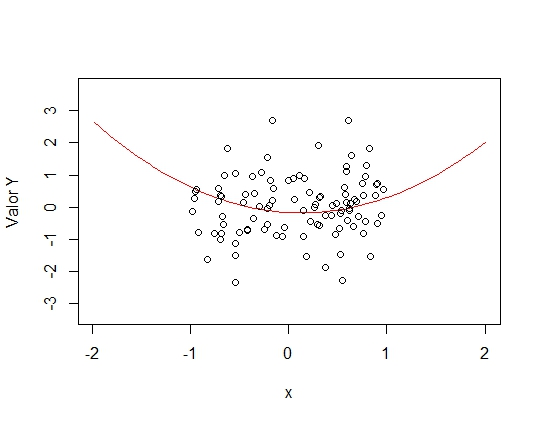
\includegraphics[width=1.0\linewidth]{captura11}
		\caption{Estimación $g_2$}
		\label{fig:captura11}
		\end{figure}
		
		\begin{figure} [H]
		\centering
		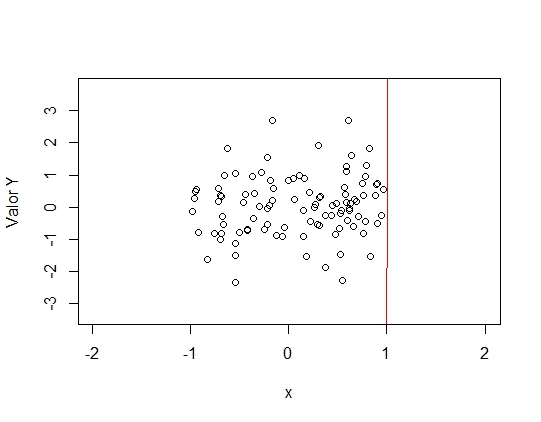
\includegraphics[width=1.0\linewidth]{captura12}
		\caption{Estimación $g_{10}$}
		\label{fig:captura12}
		\end{figure}

		Como vemos $g_2$ se ajusta mucho mejor a los datos que $g_{10}$. Esto puede deberse a que estamos estimando una función de grado 2.

		\item  ¿Por qué normalizamos $f$? (Ayuda: interpretar el significado de $\sigma$)	
	\end{enumerate}
	
	\section{Regularización y selección de modelos}
	\subsection{Ejercicio 1}
	 Para $d=3$ (dimensión) generar un conjunto de $N$ datos aleatorios $\{fx_n,y_n\}$ de la siguiente forma. Para cada punto $x_n$ generamos sus coordenadas muestreando de forma independiente una ${\cal{N}}(0,1)$. De forma similar generamos un vector de pesos de (d+1) dimensiones $w_f$, y el conjunto de valores $y_n=fw_f^Tfx_n+\sigma\epsilon_n$, donde $\epsilon_n$ es un ruido que sigue también una ${\cal{N}}(0,1)$ y $\sigma^2$ es la varianza del ruido; fijar $\sigma=0.5$.
	 
	 Usar regresión lineal con regularización ``weight decay'' para estimar $fw_f$ con $w_{reg}$. Fijar el parámetro de regularización a $0.05/N$.
	 \begin{enumerate}
	 	\item Para $N\in\{d+15,d+25,...,d+115\}$ calcular los errores $e{1},...,fe{N}$ de validación cruzada y $Ecv$.
	 	\\
	 	\\
	 	
	 	Para calcular los distintos $e_i$ lo que hago es una validación 'leave-one-out', que consiste en dejar un dato fuera del data set para estimar la función $g$ y validar esta función (averiguar el error) con este dato eliminado del training set. Este proceso tengo que repetirlo para cada uno de los datos del data set.
	 	\\
	 	\\
	 	
	 	Para obtener los pesos con regularización, empleo la expresión: 
	 	$$w_{reg} = (Z^TZ + \lambda I)^{-1}Z^Ty$$. En mi experimento obtengo los siguientes valores para el error de validación cruzada ($E_{cv}$):
	 	\begin{figure} [H]
		\centering
		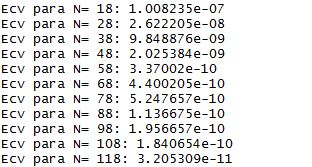
\includegraphics[width=0.7\linewidth]{captura13}
		\caption{$E_{cv}$}
		\label{fig:captura13}
		\end{figure}

	 	\item Repetir el experimento $10^3$ veces, anotando el promedio y la varianza de $e{1}$, $e{2}$ y $Ecv$ en todos los experimentos.
	 	\\
	 	\\
	 	
	 	Este experimento está implementado en el script.
	 	\\
	 	\\
	 	
    \item ¿Cuál debería de ser la relación entre el promedio de los valores de $e{1}$ y el de los valores de $E_{cv}$ ? ¿y el de los valores de $e{2}$? Argumentar la respuesta en base a los resultados de los experimentos.
    \item ¿Qué es lo que contribuye a la varianza de los valores de $e{1}$ ? \\
    Lo que contribuye a la varianza es el hecho de que los $e_1$ cambien de un experimento a otro.
	 \end{enumerate}
	 \end{document}
\end{document}